\chapter{Algorithm extensions}

The abstract algorithm presented in the previous chapter could be na\"{\i}vely implemented, yet doing so will most likely result in an implementation that does not fulfill the real-time constraint present on a mobile robot.

The extensions introduced in this chapter attempt to lower the computational requirements. They include a \textit{coarse-to-fine refinement} scheme which locally limits both the error stack layer count and the minimum error search space, as well as the calculation of so called \textit{flow templates} which contain precalculated motion field vectors.

\section{Coarse-to-fine refinement}

\label{sec:coarse_to_fine}

This section introduces an optimization to the depth reconstruction algorithm which aims at fulfilling two --- seemingly contradictory --- goals: On the one hand preventing mismatches in the depth reconstruction caused by temporal aliasing and on the other hand lowering the runtime requirements.

First some further motivation and the general idea will be given, followed by remarks regarding the concrete implementation.

\subsection{Motivation: temporal aliasing}

Reconstructing optical flow is prone to \textit{temporal aliasing}\footnote{A well known example for temporal aliasing is often seen in movies, where the so called \textit{wagon-wheel effect} causes wagon wheels to be seemingly spinning into the wrong direction \citep{wiki:WagonWheel}.}: As a consequence of the Nyquist-Shannon sampling theorem \citep[see][]{wiki:samplingTheorem}, the motion of a regular pattern with a maximum spatial frequency $\xi$ moving at a certain velocity $v$ can only be uniquely reconstructed from a time series of images, if the sampling time $T$ fulfills the following inequality
\begin{equation}
  T \leq \frac{1}{2B} = \frac{1}{2 v \xi}
  \label{eqn:spatial_shannon}
\end{equation}
where $B = v \cdot \xi$ is the maximum temporal frequency in the system.

In the optical flow case, all three variables $T, \xi$ and $v$ are fixed: $T$ is the maximum time between two snapshots, the spatial frequency $\xi$ is bounded by the image resolution and the maximum landmark velocity $v$ is defined by the minimum landmark distance and the maximum observer velocity.

For high-resolution images, the theoretically required sampling frequency turns out to be impracticably high. Conversely operating with a $T$ lying above the Nyquist-Shannon rate results in a multitude of possible solutions, as soon as a regular pattern becomes visible. Any of these solutions may produce a pronounced minimum in the global error function \ref{eqn:optical_flow}.

\subsection{Working around temporal aliasing: coarse-to-fine refinement}

Coarse-to-fine refinement as described by \citet[p. 254f., section ``Temporal Aliasing and Coarse-To-Fine Refinement'']{flowchapter05} is a solution to this problem:
\begin{enumerate}[1.]
 \item Start with the coarsest scale of a Gaussian image pyramid --- thus the maximum spatial frequency $\xi$ is small and $T$ is expected to be sufficiently large.
 \item Perform optical flow-estimation on this resolution level resulting in a vector field $\vec u$.
 \item Warp the next resolution level in the image pyramid according to $\vec u$. Subsequently the velocities $v$ are much smaller in the warped image and will outweigh the higher spatial resolution $\xi$ at this resolution level.
 \item Calculate the residual optical flow and refine the last flow vector field.
 \item Repeat step 3.\ until the highest resolution level is reached.
 \item Add up the flow vectors from all stages.
\end{enumerate}
A major problem of this approach is that a poor initial estimate cannot be corrected in subsequent steps. Yet from a theoretical point of view, lowering $\xi$ and/or $v$ is the only possible solution for temporal aliasing if a fixed $T$ is given.

\subsection{Integration of coarse-to-fine refinement into the depth reconstruction framework}

\begin{figure}[tb]
\begin{center}
  \begin{tabular}{p{0.85\textwidth} p{0.1\textwidth}}
  \subbottom[Without coarse-to-fine refinement \label{fig:temporal_aliasing_01}]{
    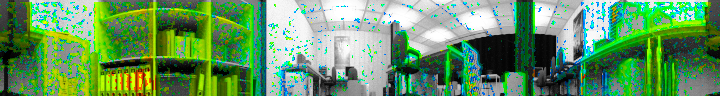
\includegraphics[width=0.825\textwidth]{media/temporal_aliasing_01.png}
  }
  \subbottom[With coarse-to-fine refinement \label{fig:temporal_aliasing_02}]{
    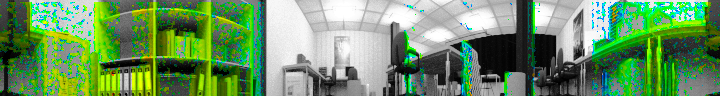
\includegraphics[width=0.825\textwidth]{media/temporal_aliasing_02.png}
  }
  &
  \subbottom[\label{fig:temporal_aliasing:scale}]{
    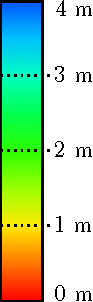
\includegraphics[width=0.08975\textwidth]{media/depth_scale_vert.pdf}
  }
  \end{tabular}
  \caption{Effects of coarse-to-fine refinement. Notice the mismatches originating from temporal aliasing in the lower left image region of (a) (book shelf). In (b) these mismatches are mostly eliminated by applying the coarse-to-fine refinement. Additionally, the pruning introduced with the coarse-to-fine refinement excludes ``uninteresting'' image regions from the depth reconstruction. As seen in the book shelf region in (b) this pruning might sometimes be oversensitive. (c) Shows the color-to-distance mapping used in the images.}
\end{center}
\end{figure}

Temporal aliasing is also a problem in the depth reconstruction algorithm and its implicit optical flow calculation. The ambiguous minima may result in high velocity flow vectors and falsely classified ``near'' objects, which in return cause false-positive obstacle points. See figure \ref{fig:temporal_aliasing_01} for an example of mismatches and the resulting depth in repetitive regions.

The coarse-to-fine approach described above is applied to the depth reconstruction algorithm as follows:
\begin{enumerate}[1.]
 \item Calculate a Gaussian pyramid for both the snapshot and the current view image. Let the number of pyramid levels be $n$.
 \item Pyramid level $\ell = 1$: Perform a complete depth reconstruction on the coarsest pyramid level resulting in the depth field $\img{R}_1(\vec p)$.
 \item Pyramid level $1 < \ell \leq n$: Perform the depth reconstruction on the next finer pyramid level. For every pixel $\vec p$, limit the search range $I_{\vec p}$ in the minimum error search to an interval around the last depth as stored in $\img{R}_{\ell - 1}(\vec p)$. This search range (given as error stack indices) could for example be chosen as
 \begin{equation}
  I_{\vec p, \ell} = \left\{\left\lceil i_\ell(\img{R}_{\ell - 1}(\vec p)) - \kappa\right\rceil, \ldots, \left\lfloor i_\ell(\img{R}_{\ell - 1}(\vec p)) + \kappa - 1\right\rfloor\right\} \cap \left\{0, \ldots, i^{MAX}_\ell\right\}
  \label{eqn:index_range_general} \; .
 \end{equation}
 The parameter $\kappa$ defines the breadth of the search range around the last index. The function $i_\ell(r)$ returns the error stack index for a certain depth value $r$ and a pyramid level index $\ell$. Note that $i_\ell(r)$ varies for all $\ell$, as the image resolution changes (due to subsampling) and so does the count of error stack layers $i^{MAX}_\ell$. This results from the fact that the maximum horizontal shift between two error stack layers is always set to one pixel (section \ref{sec:error_stack}), but the pixel resolution differs between the pyramid levels.
\end{enumerate}
Note that this approach differs from the original coarse-to-fine refinement scheme: The individual pyramid levels are not warped according to the last flow vector field. This warping was performed in order to reduce the maximum landmark velocity and to conform with the Nyquist-Shannon sampling theorem. Yet limiting the search range in the one dimensional minimum error search --- and thus the maximum flow vector length --- has the same effect.

\subsection{Implementation remarks}

\label{sec:coarse_to_fine_implementation}

\begin{figure}[t]
 \begin{center}
  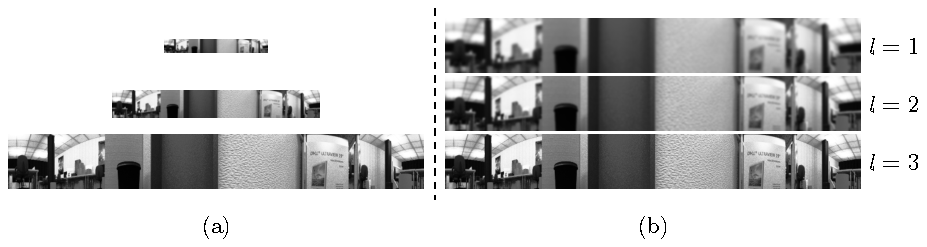
\includegraphics[width=0.975\textwidth]{media/resolution_pyramid.pdf}
 \end{center}
 \caption{Example of the resolution pyramid used in the algorithm. (a) shows the subsampled images for each pyramid level, while (b) contains the low-pass filtered images. Only octaves of the scale space are chosen, resulting in both the low-pass frequency and the image resolution (according to the Nyquist-Shannon sampling theorem) being doubled in each step.}
 \label{fig:resolution_pyramid}
\end{figure}

This section contains a few remarks regarding the actual coarse-to-fine refinement implementation.

\paragraph{Pyramid construction:} The first step in the coarse-to-fine refinement is to construct a Gaussian resolution pyramid for both the snapshot and the current view image. In contrast to the complete scale space pyramid used in SIFT \citep{Lowe04distinctiveimage}, only octaves are selected from the scale space, as depicted in figure \ref{fig:resolution_pyramid}. The scaled images are constructed by low-pass filtering the input images with a $5 \times 5$ binomial convolution kernel and then omitting even rows and columns. As a result, a subsampled image with halved width and height is generated\footnote{This behavior is implemented in the OpenCV \texttt{pyrDown} function.}. This process is repeated until the smallest resolution level is reached. In the current implementation three pyramid levels are generated, reaching from an input resolution of $720 \times 96$ pixels down to $180 \times 24$ pixels.

It is important to note that the first order derivatives of the images used for input dimensionality augmentation (see section \ref{sec:preprocessing}) have to be separately calculated for each resolution level and must not be downsampled along with the input image. This approach allows to reveal large scale gradients in the image and hence improves the matching between $\img{SS}$ and $\img{CV}$.

\paragraph{Simplified index range calculation:} Due to the convention in section \ref{sec:error_stack} to choose a maximum horizontal shift per error stack layer of one pixel, halving the width/height between two resolution pyramid levels also halves the count of error stack layers. An error stack index $i_{\ell - 1}$ in pyramid level $\ell - 1$ corresponds to the same distance $r$ as the error stack index $2  \cdot i_{\ell - 1}$ in pyramid level $\ell$. Consequently the index range equation \ref{eqn:index_range_general} can be reformulated as 
\begin{equation}
 I_{\vec p} = \{2 \cdot \img{J}_{\ell - 1}(\vec p) - \kappa, \ldots, 2 \cdot \img{J}_{\ell - 1}(\vec p) + \kappa - 1\} \cap \{0, \ldots, i^{MAX}_\ell\}
 \label{eqn:index_range} \;.
\end{equation}
Note that the unrefined index field $\img{J}$ is used, as the rounding in equation \ref{eqn:index_range_general} would undo the effects of the refinement. Consequently the index refinement and the index-to-depth steps can be skipped for all resolution layers $\ell < n$.

The concrete implementation additionally guarantees $|I_{\vec p}| = 2\kappa$. This is ensured in a correction step performed after clipping to $\{0, \ldots, i_\ell^{MAX} \}$ (not represented in the equation for sake of simplicity, see figure \ref{fig:index_ranges} instead).

\paragraph{Index range representation:}

Locally limiting the search range of each pixel turns out to be problematic from a runtime point of view. Besides the memory footprint needed for storing the index ranges it would also hinder a SIMD implementation of the minimum error search. By definition, SIMD instructions can only be used if the same operation is performed on blocks of data --- which is certainly not true if each pixel potentially needs to be compared to a different range of reference values. Even in a non-SIMD implementation, the additional branching and memory access could potentially outweigh the benefit of being capable to skip some (relatively cheap) comparisons.

A solution is to store the index range column- instead of pixelwise. The index range $I_\beta$ for column $\beta$ is then calculated as
\begin{align}
 \breve I_{\beta} &= \bigcup_{\gamma} I_{(\beta, \gamma)} \label{eqn:index_range_column_cup} \; , \\
 I_{\beta} &= \{\min(\breve I_{\beta}), \ldots, \max(\breve I_{\beta})\label{eqn:index_range_column}\} \; .
\end{align}
Using this index range for all pixels in a column may lead to problems if the indices are subject to high variance (see figure \ref{fig:index_ranges} for an example). In this case, there is no restriction in the flow vector length and the column is open to the problems caused by temporal aliasing.

\begin{figure}[tb]
 \begin{center}
  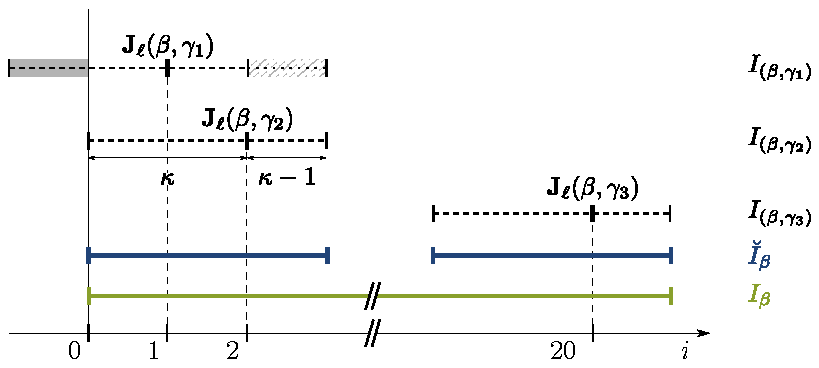
\includegraphics[width=0.975\textwidth]{media/index_ranges.pdf}
 \end{center}
 \caption{The index range calculation as stated in equations \ref{eqn:index_range_column_cup} and \ref{eqn:index_range_column}. The individual pixel index intervals from column $\beta$ are joined, resulting in the auxiliary set $\breve I_\beta$. The minimum and maximum values of $\breve I_\beta$ are then used to build the final column index range $I_\beta$. The gray areas surrounding the interval at pixel $(\beta, \gamma_1)$ visualize the ``breadth constancy'' employed in the implementation (for sake of simplicity not present in the equations). Note how high variances in the indices can cause very large index ranges.}
 \label{fig:index_ranges}
\end{figure}

\paragraph{Runtime improvements and pruning:}

\begin{figure}[h]
  \begin{center}
   \subbottom[Currentview image $\img{CV}$]{
    \begin{tabular}{c}
     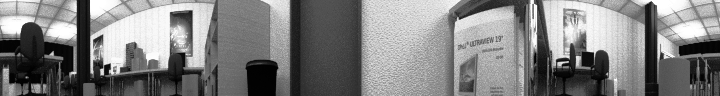
\includegraphics[width=0.9\textwidth]{media/pyramid/cv.png}
    \end{tabular}
   }
   \subbottom[Indices for $\ell = 1$, $180 \times 24$ px, $8$ error stack layers]{
    \begin{tabular}{c}
    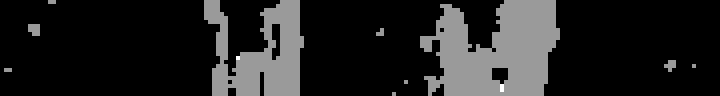
\includegraphics[width=0.9\textwidth]{media/pyramid/indices2_edited.png}\\
    
\includegraphics[width=0.9\textwidth]{media/pyramid/indexRange2.png}
    \end{tabular}
   }
   \subbottom[Indices for $\ell = 2$, $360 \times 48$ px, $16$ error stack layers]{
    \begin{tabular}{c}
    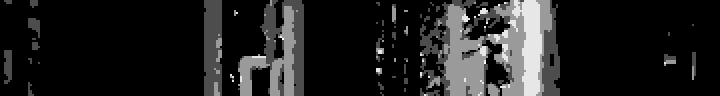
\includegraphics[width=0.9\textwidth]{media/pyramid/indices1_edited.png}\\
    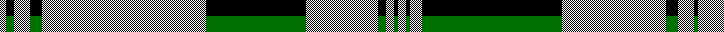
\includegraphics[width=0.9\textwidth]{media/pyramid/indexRange1.png}
    \end{tabular}
   }
   \subbottom[Refined indices for $\ell = 3$, $720 \times 96$ px, $32$ error stack layers]{
    \begin{tabular}{c}
    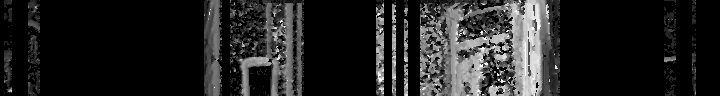
\includegraphics[width=0.9\textwidth]{media/pyramid/indices0_edited.png}\\
    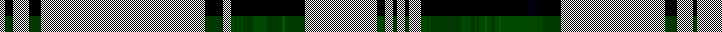
\includegraphics[width=0.9\textwidth]{media/pyramid/indexRange0.png}
    \end{tabular}
   }
  \end{center}
  \caption{Exemplary visualization of the coarse-to-fine refinement. (a) shows the reference current view image. (b)-(d) show the indices resulting from the depth reconstruction algorithm in varying resolutions. In contrast to the last resolution level in (d), the index fields in (b) and (c) have no index refinement applied to them. The small images visualize the index range of each individual column. The first (in this case black) row depicts the start index, the second (green) row the end index encoded as brightness relative to the total count of error stack layers. Note how the relative percentage of used error stack layers decreases with each resolution level. The gray/checkered regions depict pruned columns.}
  \label{fig:coarse_to_fine_pyramid}
\end{figure}

The coarse-to-fine refinement leads to a significant reduction of the runtime as the error stack layers only need to be calculated in the regions actually required for higher resolution levels.

An additional runtime optimization is given by pruning ``uninteresting'' parts of the image from the error stack calculation and the minimum error search (see also figure \ref{fig:coarse_to_fine_pyramid}). ``Uninteresting'' hereby refers to image regions containing no close obstacles. This can be easily accomplished by excluding all image columns $\beta$ from the calculation where $\img{J}_{\ell}(\beta, \gamma) = 0 \; \forall \; \gamma$.

Possibly undesired effects of this pruning can be seen in figure $\ref{fig:temporal_aliasing_02}$, where on the one hand noise is greatly reduced, but on the other hand interesting parts (although with a relatively high distance) are also pruned.

\section{Flow template calculation}

\label{sec:flow_template_calculation}

The most important concept in the optimized implementation of the abstract depth reconstruction algorithm is the computation of so-called ``flow templates''. In essence these contain the precomputed motion field vectors which are needed to warp the snapshot images. 

\subsection{Motion field parameter space reduction}

\begin{figure}[tbp]
\begin{center}
 \subbottom[Plot of $\vec u(\vec p; T(d, \alpha, \psi), r)$ for $d = 0.1 \; \mathrm{m}$, $\alpha = 0.0$, $\psi = 0.0$, $r = 1.0 \; \mathrm{m}$]{
 \includegraphics[width=0.975\textwidth]{{media/flow/flow_lines_d0.10_alpha0.00_psi0.00_r1.00}.pdf}}
 \subbottom[Plot of $\vec u(\vec p; T(d, \alpha, \psi), r)$ for $d = 0.0 \; \mathrm{m}$, $\alpha = 0.0$, $\psi = 0.1$, $r = 1.0 \; \mathrm{m}$]{
 \includegraphics[width=0.975\textwidth]{{media/flow/flow_lines_d0.00_alpha0.00_psi0.10_r1.00}.pdf}}
 \subbottom[Plot of $\vec u(\vec p; T(d, \alpha, \psi), r)$ for $d = 0.1 \; \mathrm{m}$, $\alpha = 0.0$, $\psi = 0.1$, $r = 1.0 \; \mathrm{m}$]{
 \includegraphics[width=0.975\textwidth]{{media/flow/flow_lines_d0.10_alpha0.00_psi0.10_r1.00}.pdf}}
 \subbottom[Plot of $\vec u(\vec p; T(d, \alpha, \psi), r)$ for $d = 0.1 \; \mathrm{m}$, $\alpha = 1.0$, $\psi = 0.0$, $r = 1.0 \; \mathrm{m}$]{
 \includegraphics[width=0.975\textwidth]{{media/flow/flow_lines_d0.10_alpha1.00_psi0.00_r1.00}.pdf}}
\end{center}
\caption{Plots of the motion field $\vec u(\vec p; T(d, \alpha, \psi), r)$ for varying parameters. (a) Shows a pure translatory movement, with focus of expansion (FOE) at $\beta = 0$ and focus of contraction (FOC) at $\beta = \pi$. (b) Shows a pure rotational movement. (c) Shows the combination of both the translatory and the rotational movement. Note how the to motion fields from (a) and (b) are just additively combined. (d) Shows a pure translatory movement with $\alpha \neq 0$. Note how the FOE at $\beta = \alpha$ and FOC at $\beta = \alpha + \pi$ correspond to the movement direction defined by $\alpha$. This is equivalent to a coordinate transformation in $\beta$.}
\label{fig:motion_field_plots}
\end{figure}

Calculating the motion field $\vec u(\vec p; T(d, \alpha, \psi), r)$ for each set of motion parameters $d, \alpha, \psi$, depth step $r_i$ and pixel $\vec p = (\beta, \gamma)$ as stated in the abstract algorithm is not reconcilable with the real-time constraint, as the motion field equation contains numerous trigonometric functions which are relatively slow to evaluate due to their transcendental nature. However, precalculating the motion field vectors in the given form is infeasible as a six-dimensional parameter space $(\beta, \gamma, d, \alpha, \psi, r)$ has to be covered. Consequently the parameter space dimensionality needs to be reduced.

The parameters $d$ and $r$ are not independent. In fact, the flow vector field only depends on the ratio of the two parameters. A graphical motivation can be seen in figure \ref{fig:cylinder_coordinates_transformation}, where the flow vector depends on the triangle formed by $r$ and $d$. Scaling this triangle does not change the flow vector. A proof is given in appendix \ref{proof:flow_subst}. Thus a new parameter $\rho$ can be introduced which expresses the ratio between the two values:
\begin{equation}
 \vec u(\vec p; T(d, \alpha, \psi), r) = \vec u(\vec p; \alpha, \psi, \rho) \text{ where } \rho := \frac{d}{r} \; .
\end{equation}
This substitution was originally presented in the related warping algorithm for visual homing \citep{franz1998did}.

\paragraph{Eliminating the rotational movement:} The motion parameters $\alpha$ and $\psi$ describe the rotational movement that was executed by the robot. It can be shown (see \ref{proof:rot_motion_elim} for a proof), that varying $\alpha$ applies an affine coordinate transformation to the $\beta$-component and $\psi$ is an additive term on the $\beta$ component:
\begin{equation}
 \vec u(\vec p; \alpha, \psi, \rho) = \vec u(\vec p - (\psi + \alpha, 0)^T; \rho) - (\psi, 0)^T
 \label{eqn:rot_motion_elim} \; .
\end{equation}
See figure \ref{fig:motion_field_plots} for an example. This equation can be interpreted as elimination of the rotational movement by panoramic image alignment:
\begin{itemize}
 \item $\psi$ expresses the change in orientation between $\img{SS}$ and $\img{CV}$. Due to the nature of the panoramic images, this change in orientation can be eliminated by a simple horizontal translation of the snapshot image $\img{SS}$.
 \item $\alpha$ denotes the movement direction and by implication the position of the focus of expansion (FOE) in the image. Accordingly, $\alpha$ can be set to zero, if both the snapshot $\img{SS}$ and current view $\img{CV}$ are shifted by $\alpha$ in such a way that the observed FOE and FOC (focus of contraction) positions in $\img{CV}$ match their positions in the non-rotated motion field.
\end{itemize}
Hence using correct image alignment allows to reduce the parameter space by setting $\alpha = \psi = 0$. The resulting motion field equation becomes:
\begin{equation}
  \vec u((\beta, \gamma)^T; \rho)
  = \begmat
    \atantwo
      \left(\sin(\beta), \cos(\beta) + \rho\right) - \beta \\
    \arctan
      \left(
	\frac{
	\tan(\gamma)
      }{
      \sqrt{
    (\cos(\beta) + \rho)^{2} +
    \sin(\beta)^{2}}
      }
    \right) - \gamma
  \finmat
  =
  \begmat
    \beta' - \beta \\
    \gamma' - \gamma
  \finmat
  \label{eqn:flow_template} \; .
\end{equation}
It should be noted that the $\beta$-component of $\vec p_{\img{SS}} = (\beta', \gamma')^T$ does not depend on $\gamma$: For a constant $\rho$, all pixels in a column in $\img{SS}$ are mapped to a single column in $\img{CV}$, yet a non-linear scaling in $\gamma$-direction is applied. This property will allow the linear interpolation needed for calculating the warped $\img{SS'}_i$ to be separated into a horizontal and a vertical interpolation step (see section \ref{sec:motion_field_separability}).

\subsection{Parameter selection, index to depth conversion and distance variance}

\label{sec:index_to_depth}

\paragraph{Flow template definition:} In the last two steps the parameter space was reduced to three parameters $\beta, \gamma$ and $\rho$. This allows precalculating the motion field vectors for each pixel $\vec p = (\beta, \gamma)^T$ and a set of $n$ values of $\rho_i$ where $0 \leq i \leq n - 1$. The snapshot images can then be warped according to these motion vectors, subsequently called \textit{flow templates}. A single flow template at index $i$, $\img{U}_{i}$, is a $h \times w$ matrix containing two-dimensional vectors as its entries:
\begin{equation}
  \img{U}_i(\vec p) = \vec u(\vec p; \rho_i)
  \label{eqn:flow_template_definition} \; .
\end{equation}

\paragraph{Selection of $\rho_i$:} In section \ref{sec:error_stack} it was stated that the $r_i$ should be chosen in such a way that the maximum horizontal shift between two consecutive motion fields is about one pixel. This was motivated by the ability to exploit the complete horizontal resolution that is available in the images.

In the new motion field equation, the motion vector length in pixels solely depends on the parameter $\rho$. Thus the $\rho_i$ have to be selected with the same consideration. As shown in appendix \ref{proof:max_horz_shift} choosing, $\rho_i$ as a multiple of the horizontal angular image resolution (with $w$ being the image width in pixels)
\begin{equation}
  \rho_i = \frac{2 \pi}w \cdot i
\end{equation}
approximately fulfills this requirement for small $i$. Note that for large $i$ this means that the ``one pixel per step'' condition might by violated. In practice $d$ should always be significantly smaller than $r$, as the algorithm is designed for short distances between consecutive snapshot images. Large $d$ would imply near landmarks to be viewed from two completely different directions in the $\img{SS}$, $\img{CV}$ pair.

\paragraph{Index to depth conversion:} The distance function $r(j)$ needed for conversion from continuous index- to world-space is now given as
\begin{equation}
  r(j; d) = \frac{d}{\rho(j)} = \frac{d}j \cdot \frac{w}{2 \pi} \; .
\end{equation}


\paragraph{Calculation of $\sigma_r$:} The choice of $\sigma_r$ was left open in section \ref{sec:prob_landmarks}. Now that the index-to-depth function $r(j)$ has been selected, the corresponding variance $\sigma_r$ can be calculated, which is proportional to the error $\Delta r(j)$. Assuming an index-space error $\Delta j$ and eliminating $j$ yields:
\begin{equation}
  \Delta r(j) = \left| \frac{\partial r(j)}{\partial j} \right| \cdot \Delta j = \frac{d}{j^2} \cdot \Delta j \cdot \frac{w}{2 \pi} = \frac{r(j)^2}{d} \cdot \Delta j \cdot \frac{2 \pi}{w}
\end{equation}
Thus the variance $\sigma_r$ quadratically depends on $r$:
\begin{equation}
\sigma_r \propto \frac{r^2}{d} \label{eqn:sigma_r}
\end{equation}
